%
% $RCSfile: design.tex,v $
%
% Copyright (c) 2004. Christian Heller. All rights reserved.
%
% No copying, altering, distribution or any other actions concerning this
% document, except after explicit permission by the author!
% At some later point in time, this document is planned to be put under
% the GNU FDL license. For now, _everything_ is _restricted_ by the author.
%
% http://www.cybop.net
% - Cybernetics Oriented Programming -
%
% http://www.resmedicinae.org
% - Information in Medicine -
%
% @author Christian Heller <christian.heller@tuxtax.de>
%

\subsubsection{Design}
\label{design_heading}

Gamma et al. \cite{gamma1995} define a design pattern as: \textit{description of
collaborating objects and classes which are taylored to solve a general design
problem in a special context.} Mostly, patterns are in relation to each other.
They can be combined to master more complex tasks.

%
% $RCSfile: command.tex,v $
%
% Copyright (C) 2002-2008. Christian Heller.
%
% Permission is granted to copy, distribute and/or modify this document
% under the terms of the GNU Free Documentation License, Version 1.1 or
% any later version published by the Free Software Foundation; with no
% Invariant Sections, with no Front-Cover Texts and with no Back-Cover
% Texts. A copy of the license is included in the section entitled
% "GNU Free Documentation License".
%
% http://www.cybop.net
% - Cybernetics Oriented Programming -
%
% http://www.resmedicinae.org
% - Information in Medicine -
%
% Version: $Revision: 1.1 $ $Date: 2008-08-19 20:41:05 $ $Author: christian $
% Authors: Christian Heller <christian.heller@tuxtax.de>
%

\subsubsection{Command}
\label{command_heading}
\index{Command Pattern}
\index{Action Pattern}
\index{Transaction Pattern}
\index{Signal Pattern}

\begin{figure}[ht]
    \begin{center}
        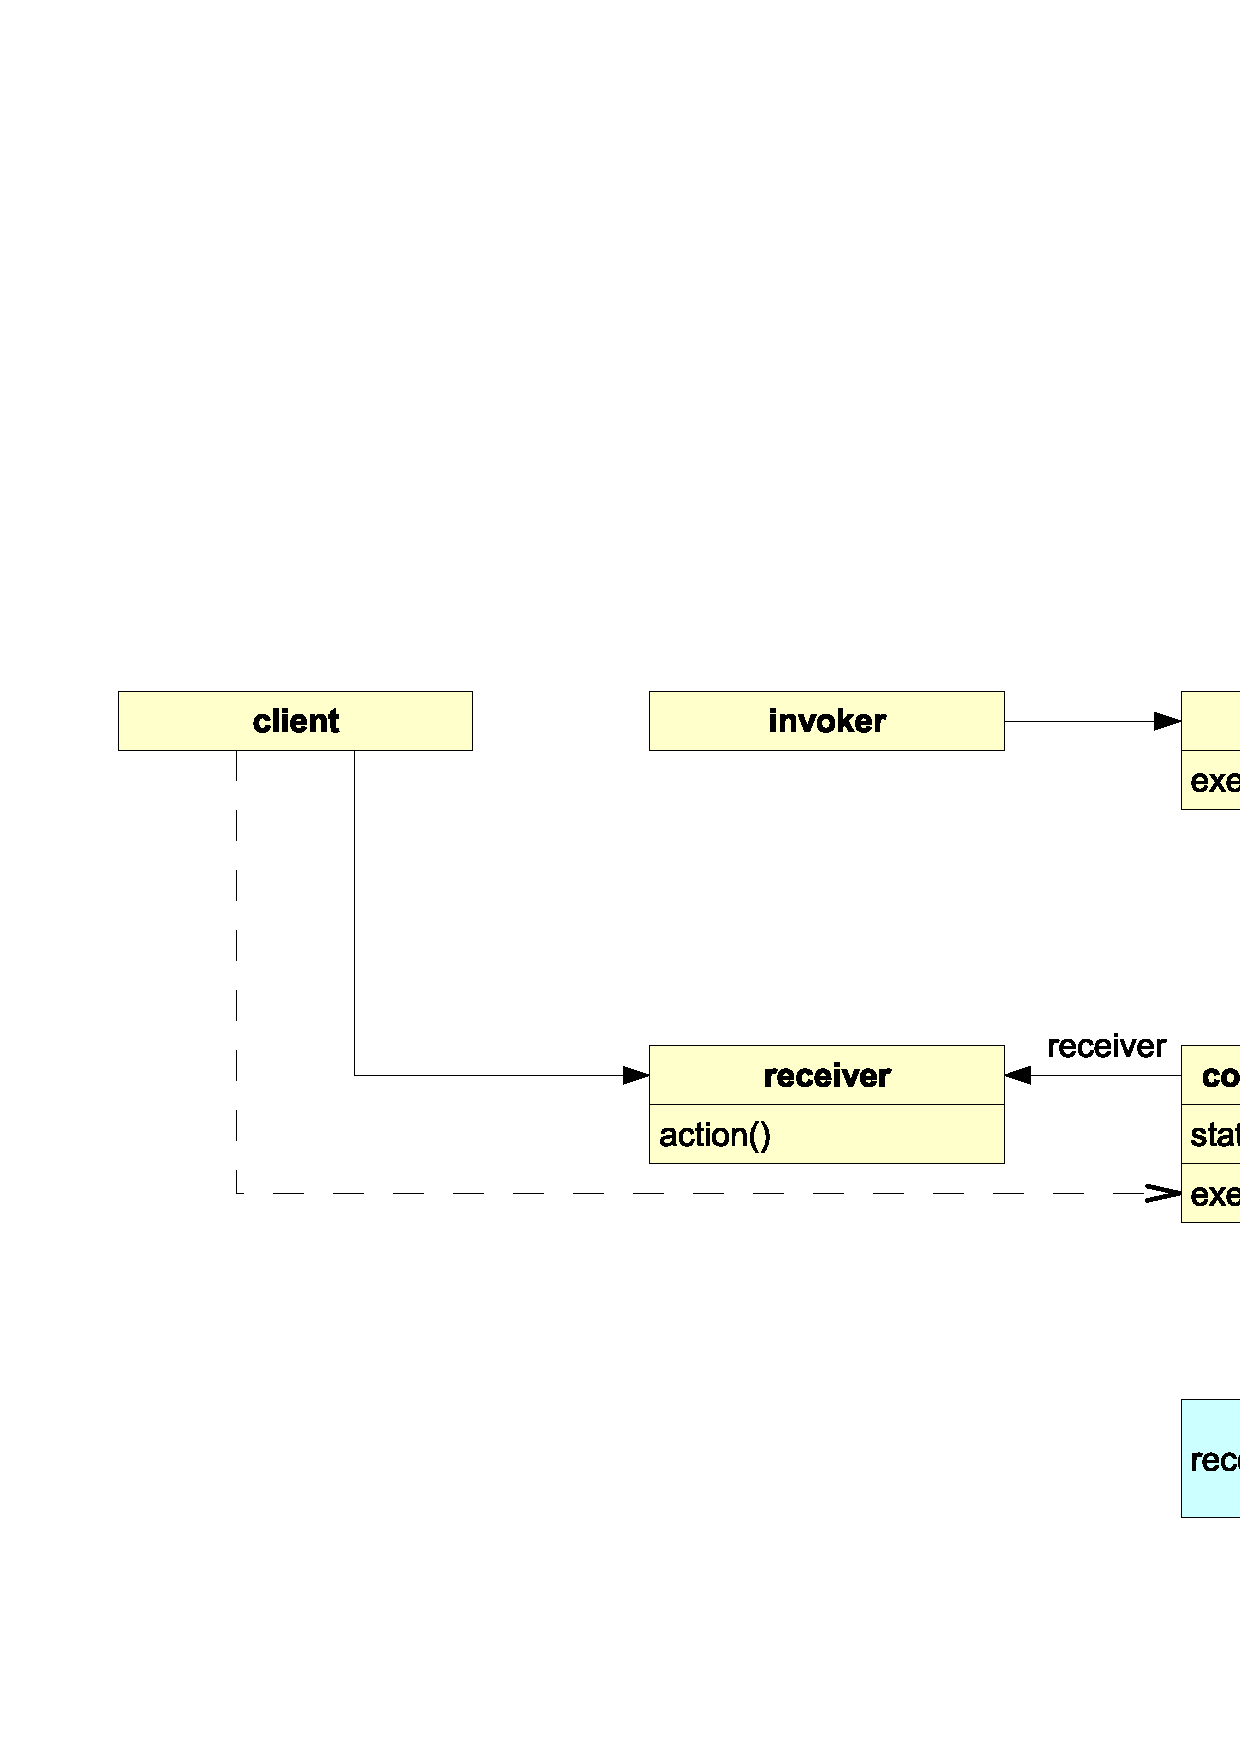
\includegraphics[scale=0.3,angle=-90]{graphic/command.pdf}
        \caption{Command Pattern}
        \label{command_figure}
    \end{center}
\end{figure}

The \emph{Command} pattern \cite{gamma1995}, also known as \emph{Action} or
\emph{Transaction}, sometimes also \emph{Signal}, encapsulates a command in
form of an object. That way, operations can get parameterised; they can be put
in a queue, be made undone or traced in a log book. Figure \ref{command_figure}
shows the structure of the pattern.

Chapter \ref{state_and_logic_heading} uses the idea of representing operations
and algorithms (logic knowledge) as independent models, similar to encapsulated
commands.

%
% $RCSfile: wrapper.tex,v $
%
% Copyright (c) 2004. Christian Heller. All rights reserved.
%
% No copying, altering, distribution or any other actions concerning this
% document, except after explicit permission by the author!
% At some later point in time, this document is planned to be put under
% the GNU FDL license. For now, _everything_ is _restricted_ by the author.
%
% http://www.cybop.net
% - Cybernetics Oriented Programming -
%
% http://www.resmedicinae.org
% - Information in Medicine -
%
% @author Christian Heller <christian.heller@tuxtax.de>
%

\paragraph{Wrapper}
\label{wrapper_heading}

The \emph{Wrapper} pattern \cite{gamma1995} allows otherwise imcompatible
classes to work together. It can be seen as skin object enclosing (wrapping) an
inner core object, to which it provides access. In other words: It adapts the
interface of a class which is why Gamma et al. call the pattern \emph{Adapter}.

\begin{figure}[ht]
    \begin{center}
        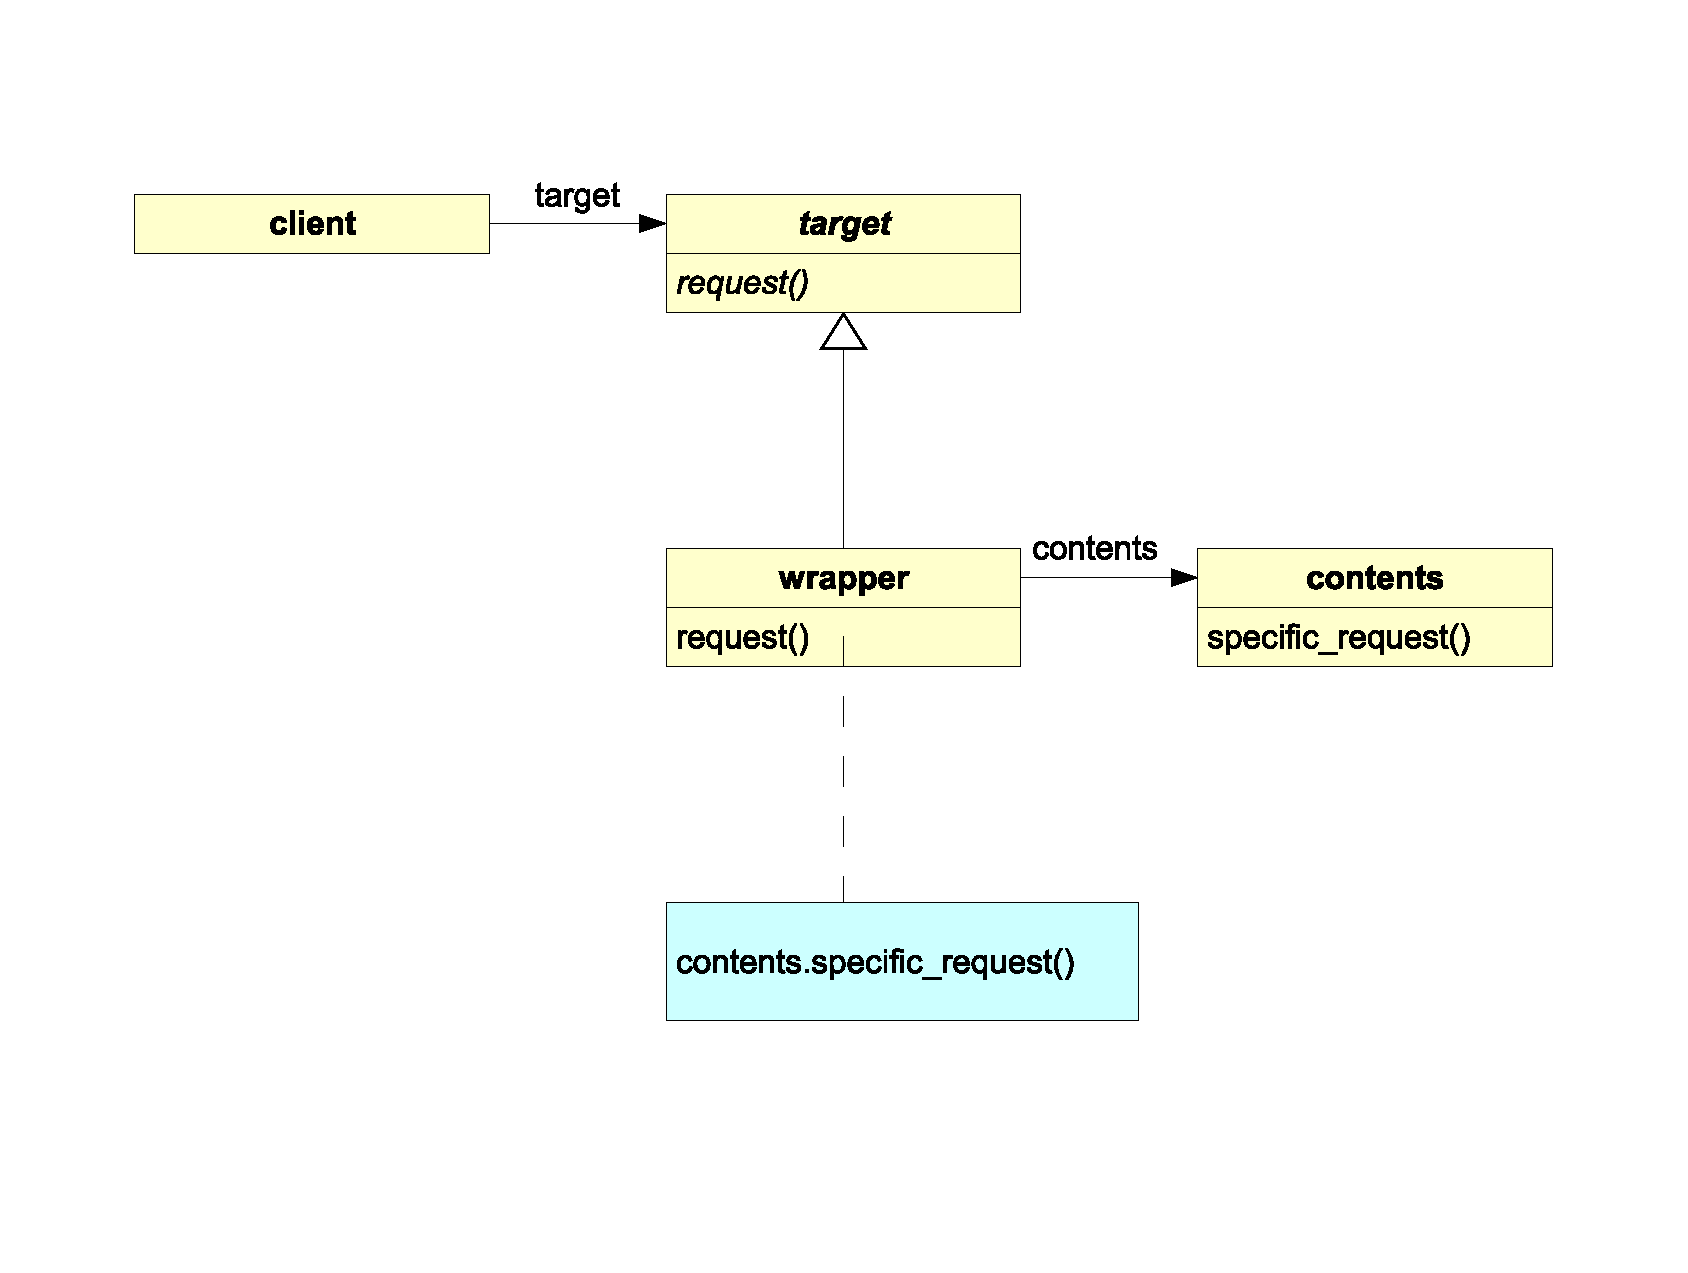
\includegraphics[scale=0.3]{vector/wrapper.eps}
        \caption{Wrapper Pattern}
        \label{wrapper_figure}
    \end{center}
\end{figure}

As can be seen in figure \ref{wrapper_figure}, this pattern makes heavy use of
\emph{Delegation}, where the \emph{Delegator} is the adapter (or wrapper) and
the \emph{Delegate} is the class being adapted \cite{portland}.

%
% $RCSfile: whole_part.tex,v $
%
% Copyright (C) 2002-2008. Christian Heller.
%
% Permission is granted to copy, distribute and/or modify this document
% under the terms of the GNU Free Documentation License, Version 1.1 or
% any later version published by the Free Software Foundation; with no
% Invariant Sections, with no Front-Cover Texts and with no Back-Cover
% Texts. A copy of the license is included in the section entitled
% "GNU Free Documentation License".
%
% http://www.cybop.net
% - Cybernetics Oriented Programming -
%
% http://www.resmedicinae.org
% - Information in Medicine -
%
% Version: $Revision: 1.1 $ $Date: 2008-08-19 20:41:09 $ $Author: christian $
% Authors: Christian Heller <christian.heller@tuxtax.de>
%

\subsubsection{Whole-Part}
\label{whole_part_heading}
\index{Whole-Part Pattern}

Whenever many components form a semantic unit, they can be subsumed by the
\emph{Whole-Part} pattern \cite{buschmann}. It encapsulates single part objects
(figure \ref{wholepart_figure}) and controls their cooperation. Part objects
are not addressable directly. Almost all software systems contain some
components or sub systems which could be organised by help of this pattern. In
some way, it is quite similar to the previously introduced \emph{Wrapper}
pattern, only that not just one but many objects are wrapped.

\begin{figure}[ht]
    \begin{center}
        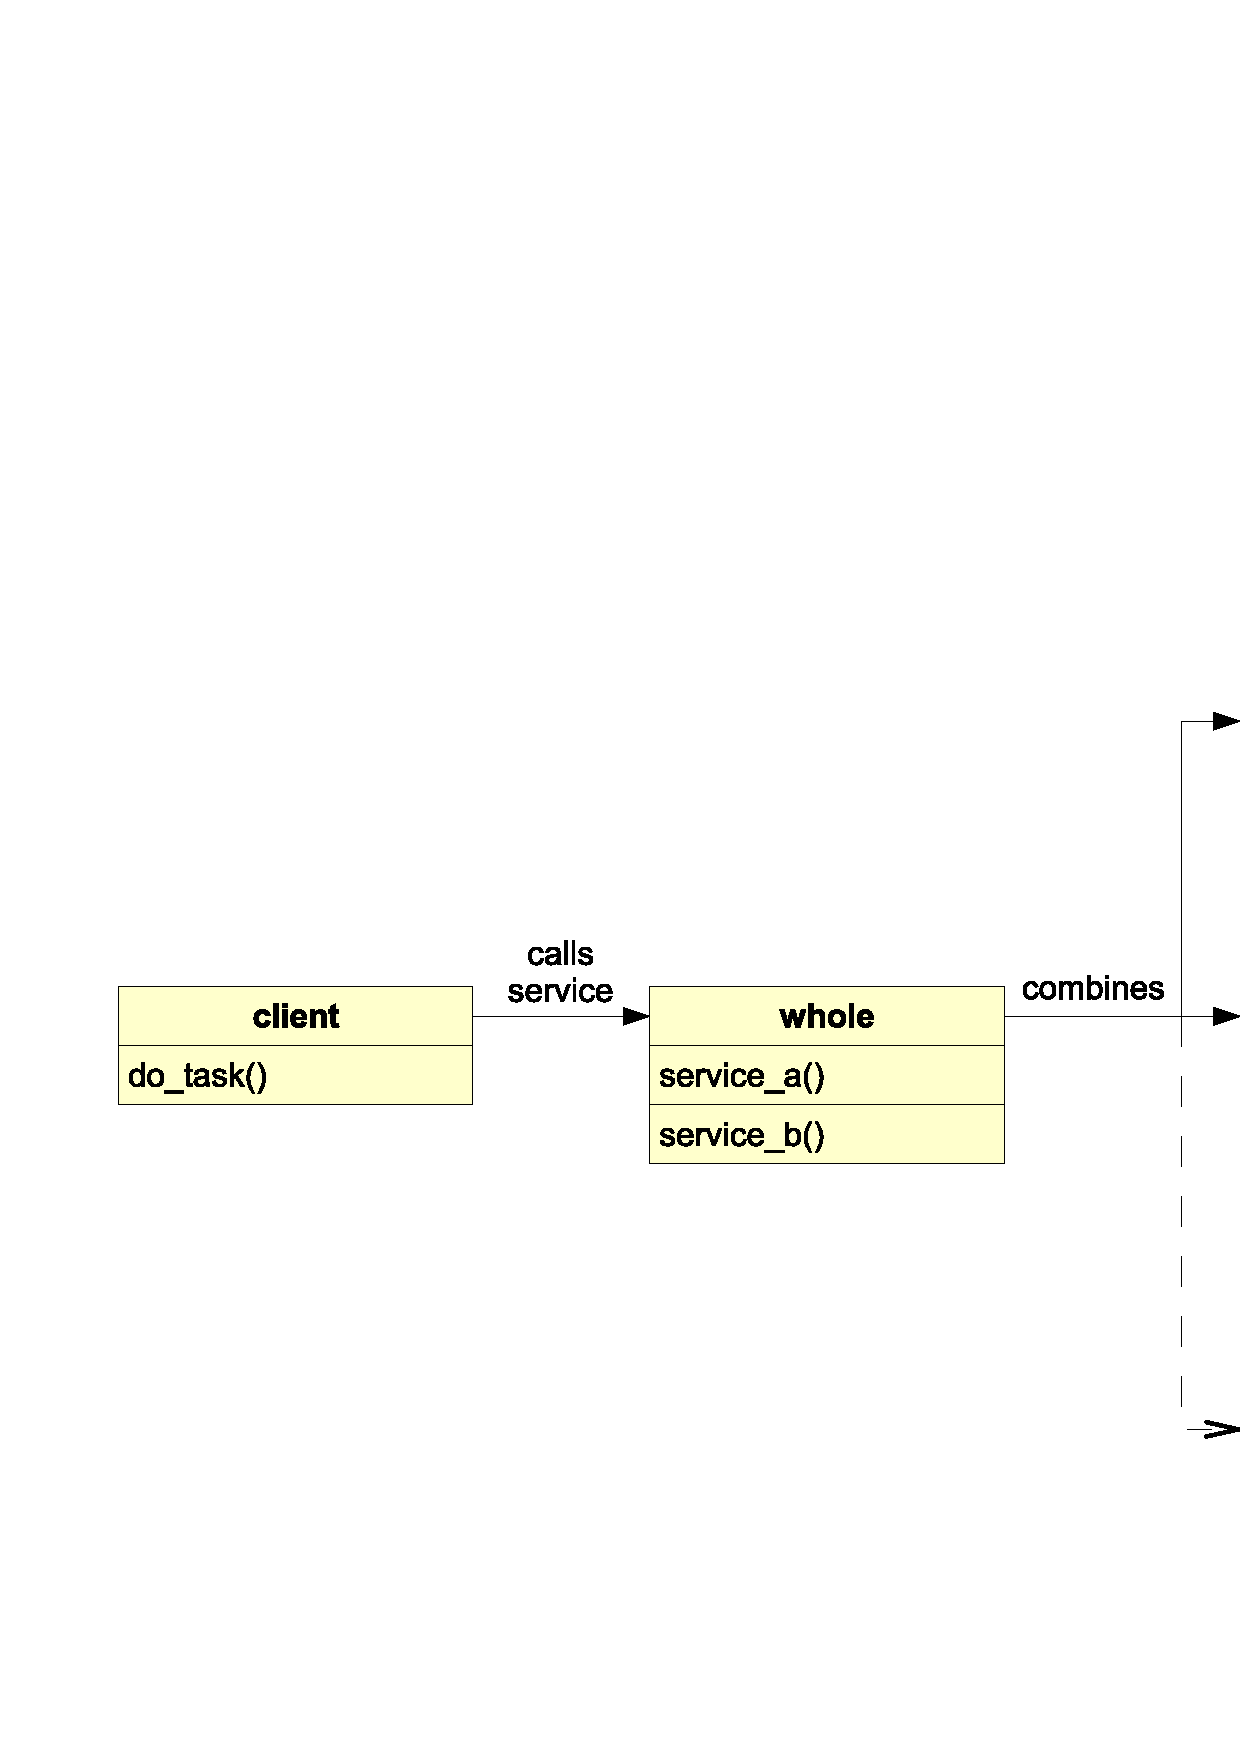
\includegraphics[scale=0.3,angle=-90]{graphic/wholepart.pdf}
        \caption{Whole-Part Pattern}
        \label{wholepart_figure}
    \end{center}
\end{figure}

The principal structure of the new language introduced in chapter
\ref{cybernetics_oriented_language_heading} is based on the \emph{Whole-Part}
pattern. One knowledge template (whole) may consist of zero, one or many other
templates (parts).

%
% $RCSfile: composite.tex,v $
%
% Copyright (C) 2002-2008. Christian Heller.
%
% Permission is granted to copy, distribute and/or modify this document
% under the terms of the GNU Free Documentation License, Version 1.1 or
% any later version published by the Free Software Foundation; with no
% Invariant Sections, with no Front-Cover Texts and with no Back-Cover
% Texts. A copy of the license is included in the section entitled
% "GNU Free Documentation License".
%
% http://www.cybop.net
% - Cybernetics Oriented Programming -
%
% http://www.resmedicinae.org
% - Information in Medicine -
%
% Version: $Revision: 1.1 $ $Date: 2008-08-19 20:41:06 $ $Author: christian $
% Authors: Christian Heller <christian.heller@tuxtax.de>
%

\subsubsection{Composite}
\label{composite_heading}
\index{Composite Pattern}
\index{Directed Acyclical Graph}
\index{DAG}
\index{Tree}
\index{Whole-Part Pattern}
\index{Recursion}

A hierarchical object structure, also called \emph{Directed Acyclical Graph}
(DAG) or \emph{Tree}, can be represented by a combination of classes called
\emph{Composite} pattern \cite{gamma1995}. It describes a \emph{Component} that
may consist of \emph{Children} (figure \ref{composite_figure}), which makes it
comparable to the \emph{Whole-Part} pattern. The difference is that the
\emph{Composite} is a more generalised version, with a dynamically extensible
number of child (part) objects. The \emph{Composite} is a pattern based on
\emph{Recursion}, which is one of the most commonly used programming techniques
at all. The pattern's split into \emph{Leaf-} and \emph{Composite} sub classes
helps distinguish primitive- from container objects. A composite tree node
holds objects of type \emph{Component}.

\begin{figure}[ht]
    \begin{center}
        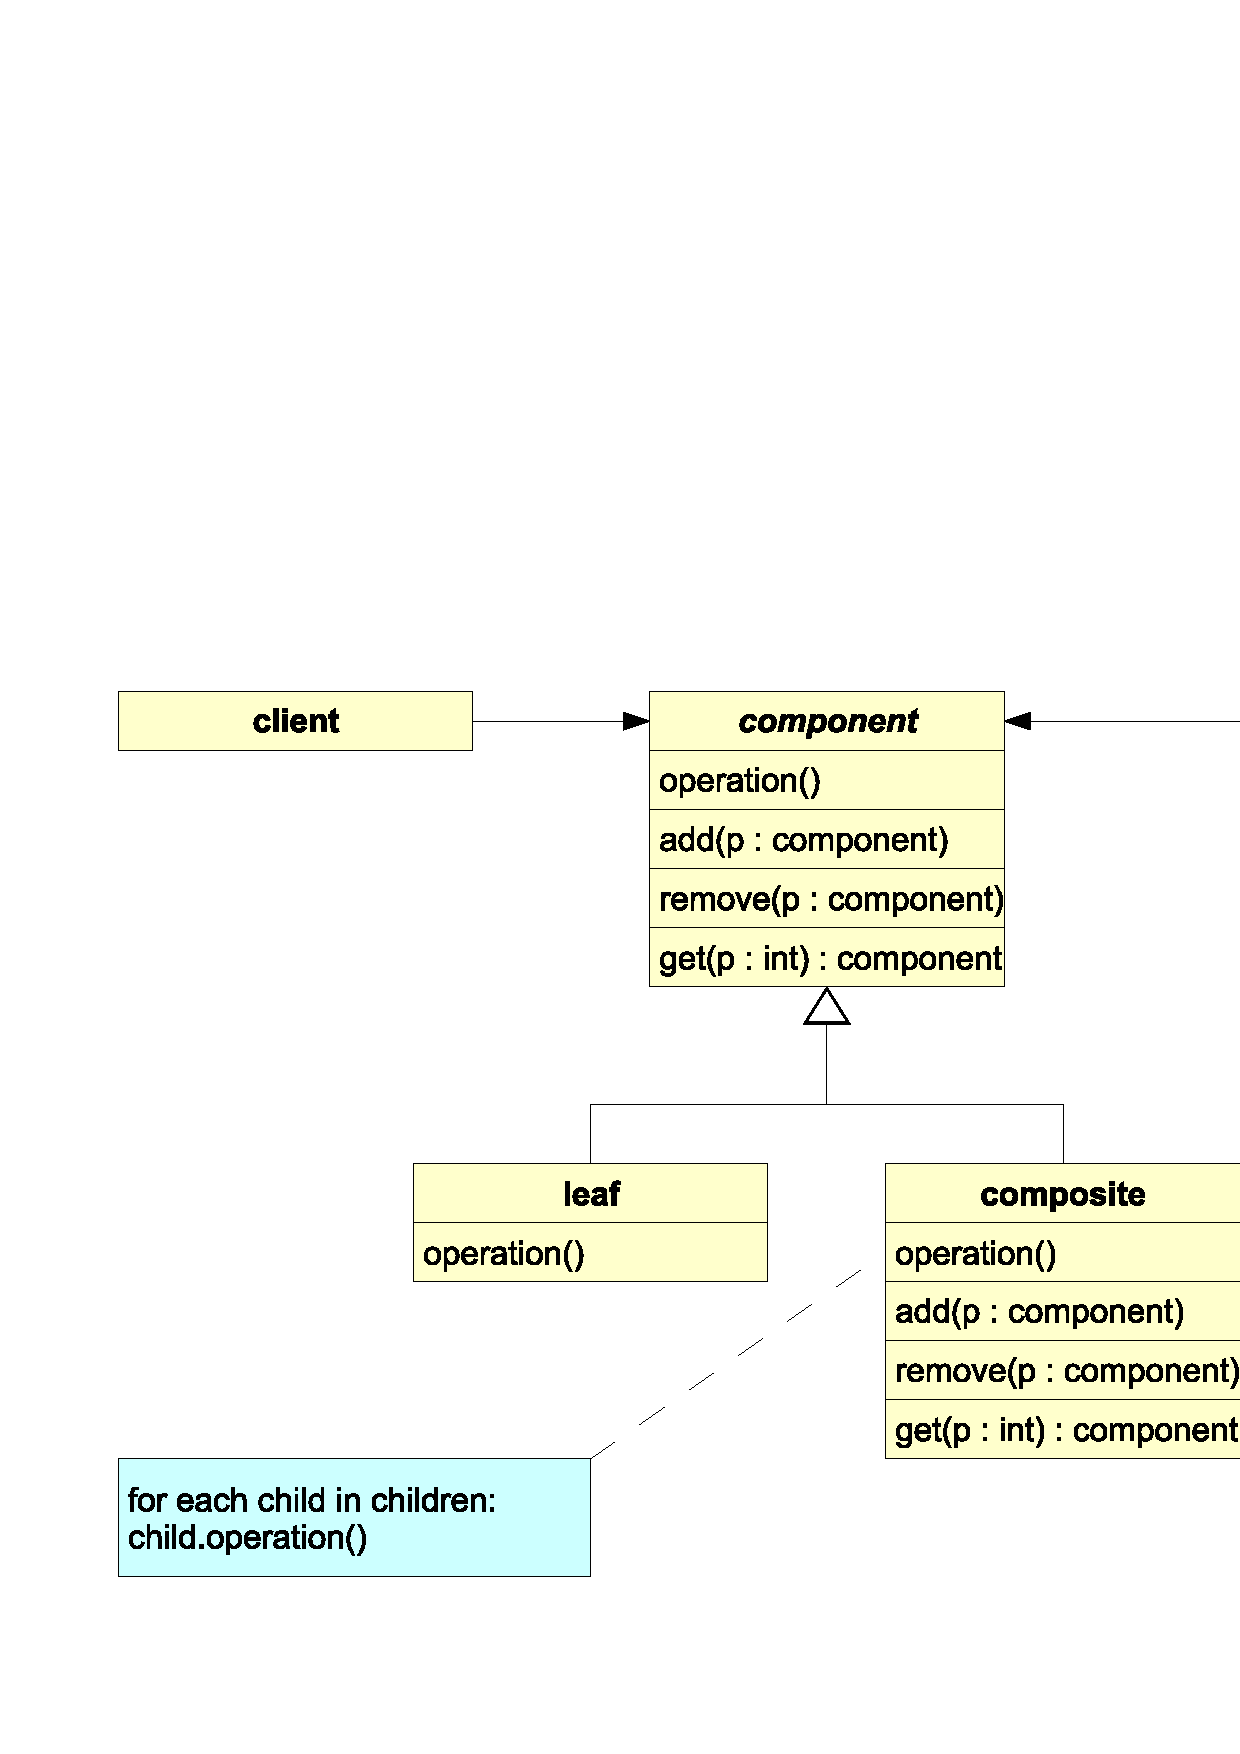
\includegraphics[scale=0.3,angle=-90]{graphic/composite.pdf}
        \caption{Composite Pattern}
        \label{composite_figure}
    \end{center}
\end{figure}

The knowledge schema introduced in chapter \ref{knowledge_schema_heading} has
container capabilities, like the composite pattern. It does, however, not
distinguish between composite and leaf nodes, and not use inheritance.

%
% $RCSfile: chain_of_responsibility.tex,v $
%
% Copyright (c) 2004. Christian Heller. All rights reserved.
%
% No copying, altering, distribution or any other actions concerning this
% document, except after explicit permission by the author!
% At some later point in time, this document is planned to be put under
% the GNU FDL license. For now, _everything_ is _restricted_ by the author.
%
% http://www.cybop.net
% - Cybernetics Oriented Programming -
%
% http://www.resmedicinae.org
% - Information in Medicine -
%
% @author Christian Heller <christian.heller@tuxtax.de>
%

\paragraph{Chain of Responsibility}
\label{chain_of_responsibility_heading}

The \emph{Chain of Responsibility} pattern \cite{gamma1995} is similar to the
\emph{Composite}, in that it represents a recursive structure as well. Objects
destined to solve a task are linked with a corresponding \emph{Successor}
(figure \ref{chain_figure}), such forming a chain. If an object is not able to
solve a task, that task is forwarded to the object's successor, along the chain.

\begin{figure}[ht]
    \begin{center}
        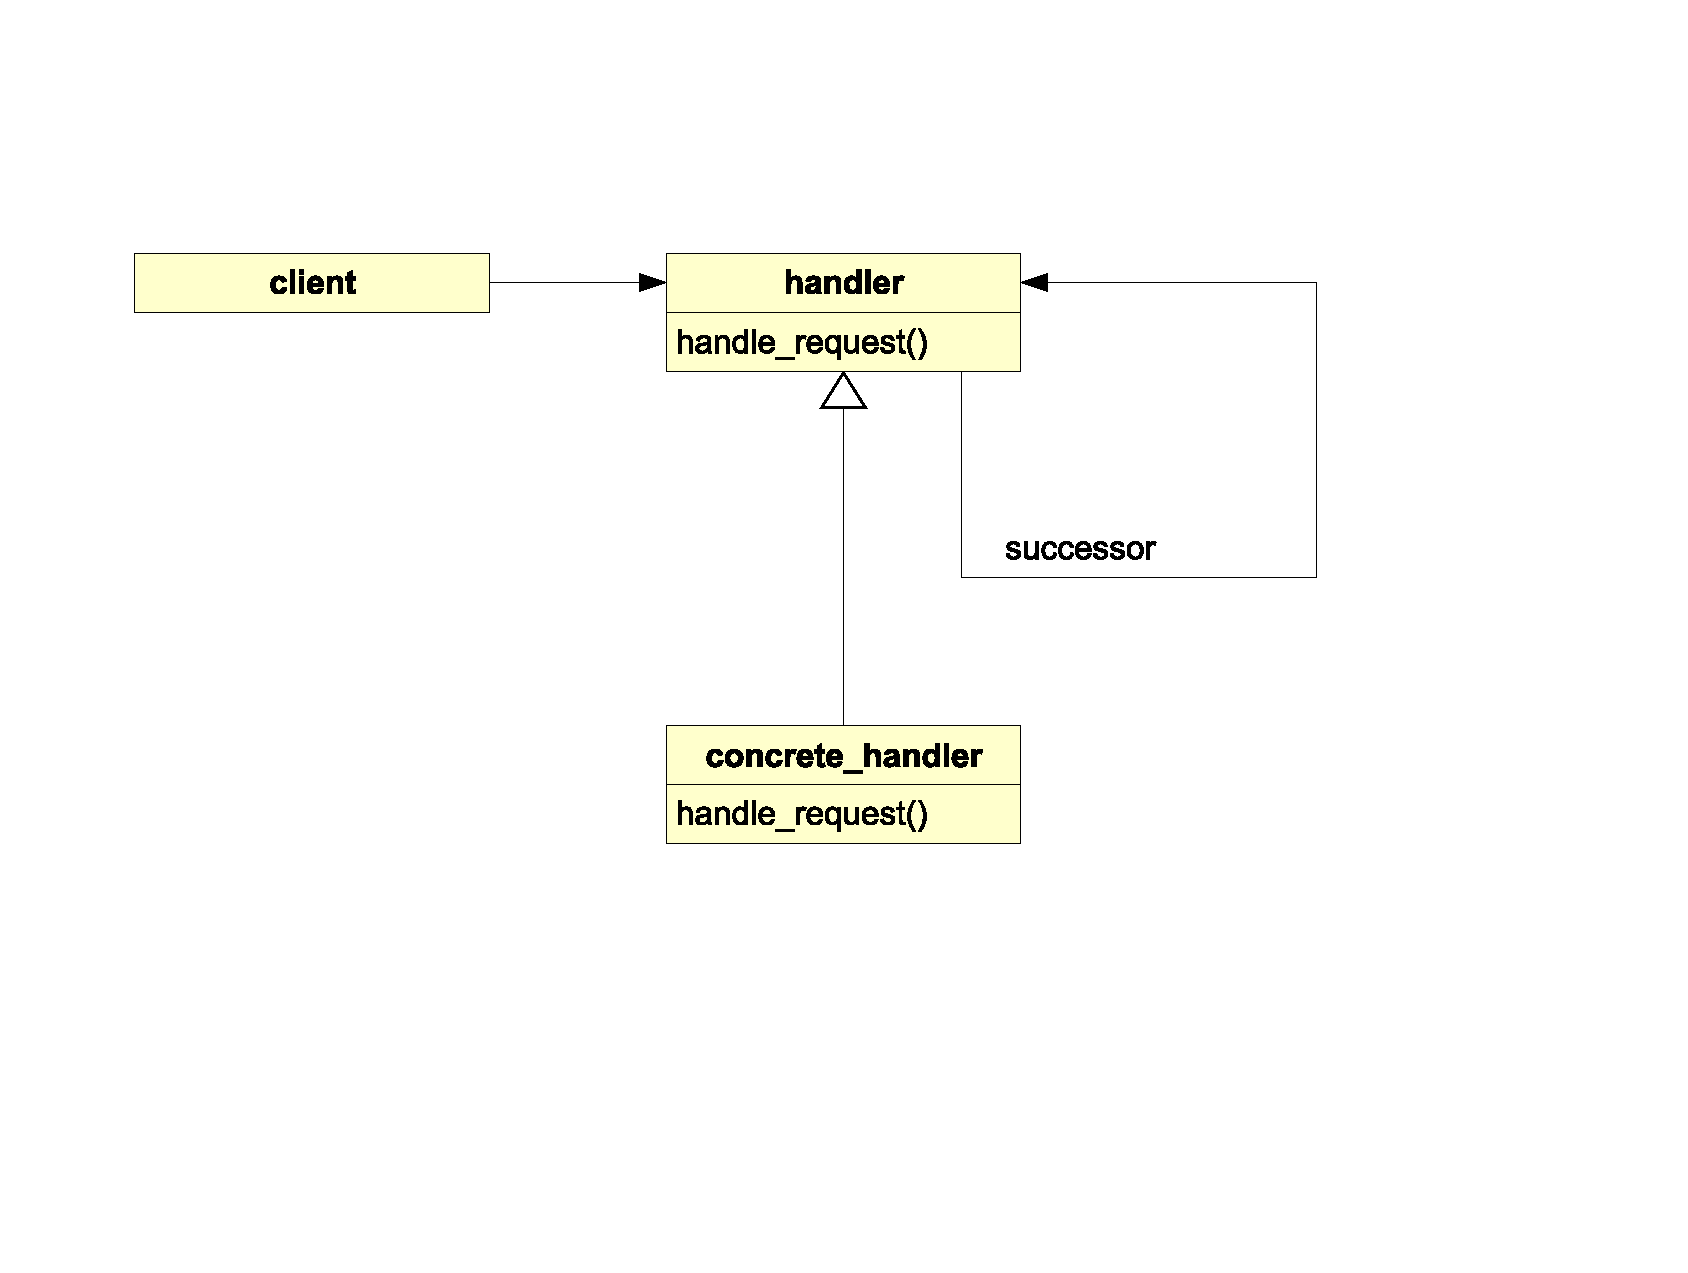
\includegraphics[scale=0.3]{vector/chain.eps}
        \caption{Chain of Responsibility Pattern}
        \label{chain_figure}
    \end{center}
\end{figure}

The pattern found wide application, for example in help systems, in event
handling frameworks or for exception handling. Its \emph{Handler} class is
known under synonyms like \emph{Event Handler}, \emph{Bureaucrat} or
\emph{Responder}.

Frequently, the pattern gets misused by delegating messages not only to children
but also to the parent of objects. The \emph{Hierarhical Model View Controller}
(HMVC) pattern is one example for this. It causes unfavourable bidirectional
dependencies (section \ref{bidirectional_dependency_heading}) and leads to
stronger coupling between the layers of a framework, because parent- and child
objects then reference each other.

%
% $RCSfile: observer.tex,v $
%
% Copyright (c) 2004. Christian Heller. All rights reserved.
%
% No copying, altering, distribution or any other actions concerning this
% document, except after explicit permission by the author!
% At some later point in time, this document is planned to be put under
% the GNU FDL license. For now, _everything_ is _restricted_ by the author.
%
% http://www.cybop.net
% - Cybernetics Oriented Programming -
%
% http://www.resmedicinae.org
% - Information in Medicine -
%
% @author Christian Heller <christian.heller@tuxtax.de>
%

\paragraph{Observer}
\label{observer_heading}

Another pattern that found wide application is the \emph{Observer} \cite{gamma1995},
an often-used synonym for which is \emph{Publisher-Subscriber}. It provides a
notification mechanism for all objects that registered as \emph{Observer} at a
\emph{Subject} in whose state changes they are interested, leading to an automatic
update of all dependent objects (figure \ref{observer_figure}).

\begin{figure}[ht]
    \begin{center}
        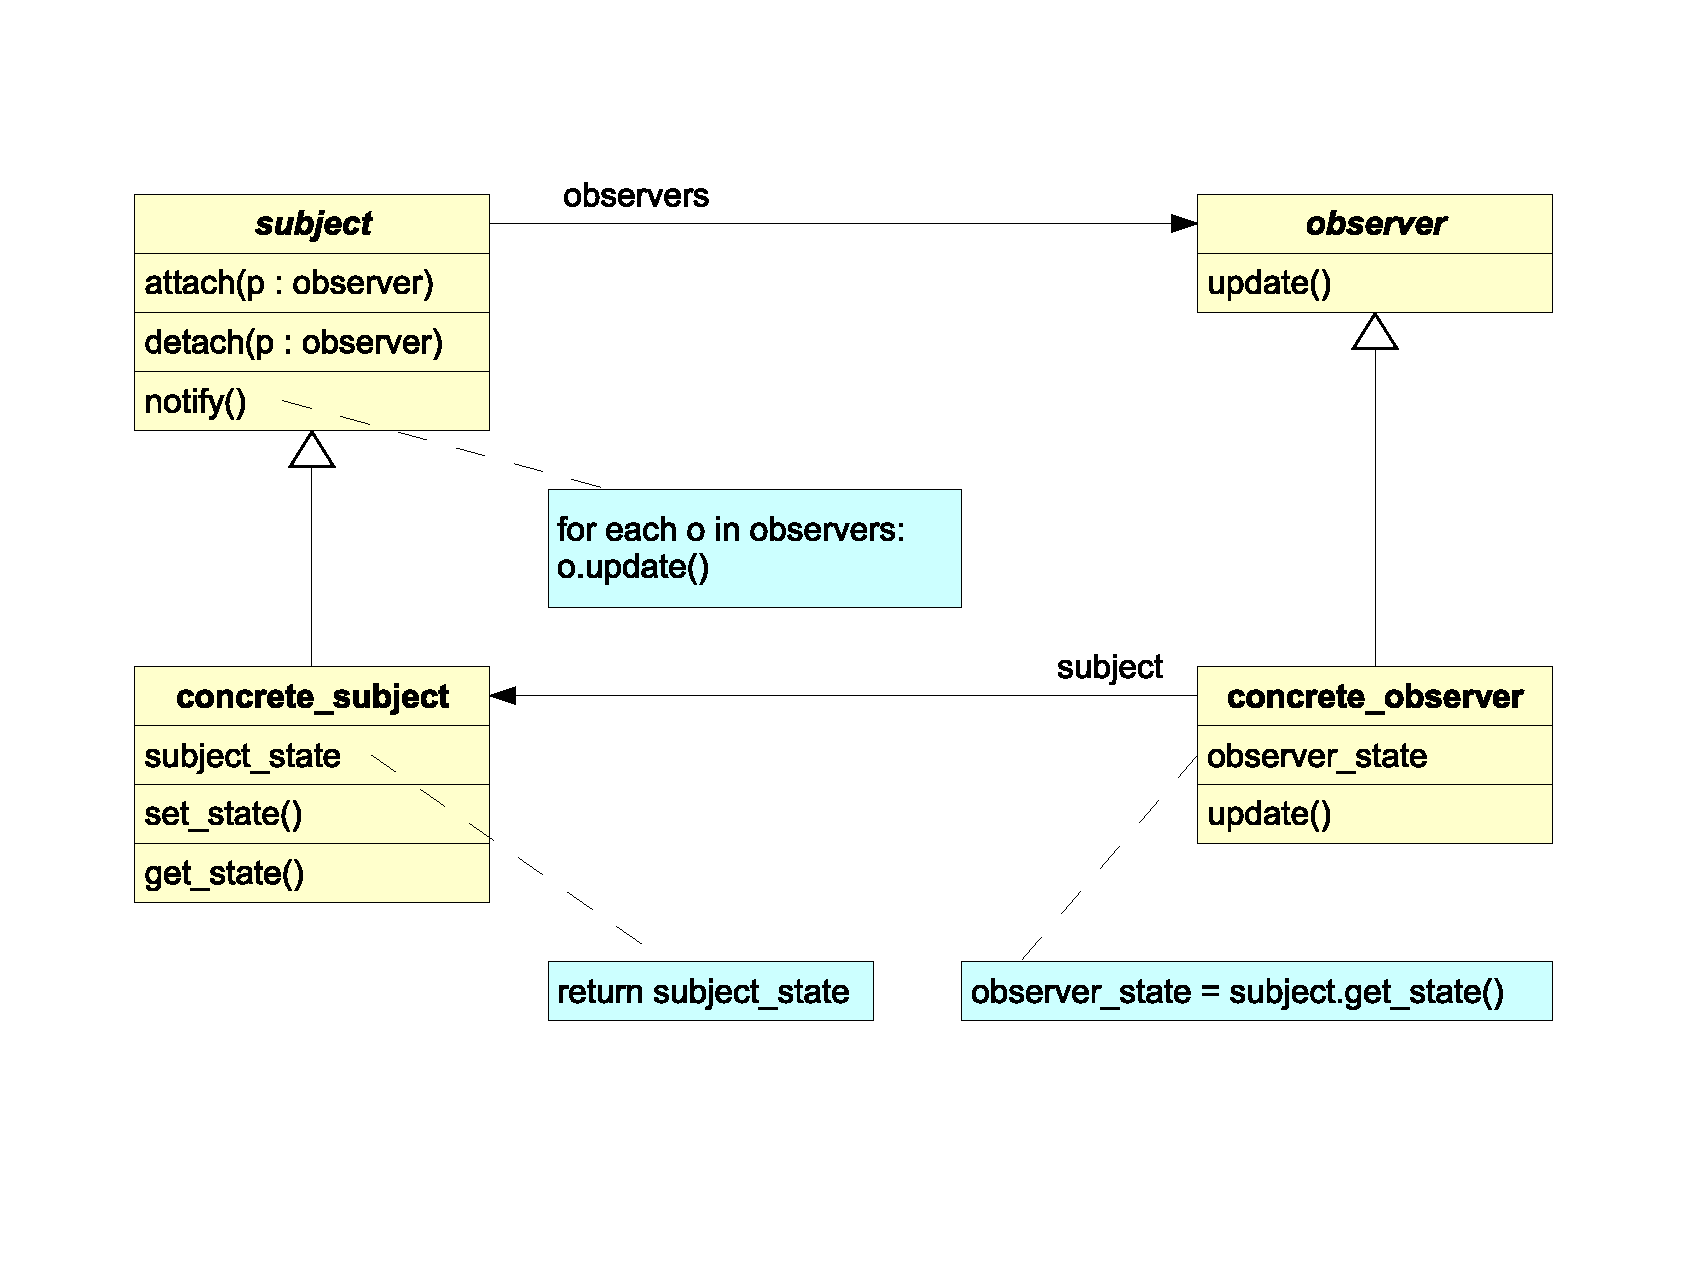
\includegraphics[scale=0.3]{vector/observer.eps}
        \caption{Observer Pattern}
        \label{observer_figure}
    \end{center}
\end{figure}

\begin{figure}[ht]
    \begin{center}
        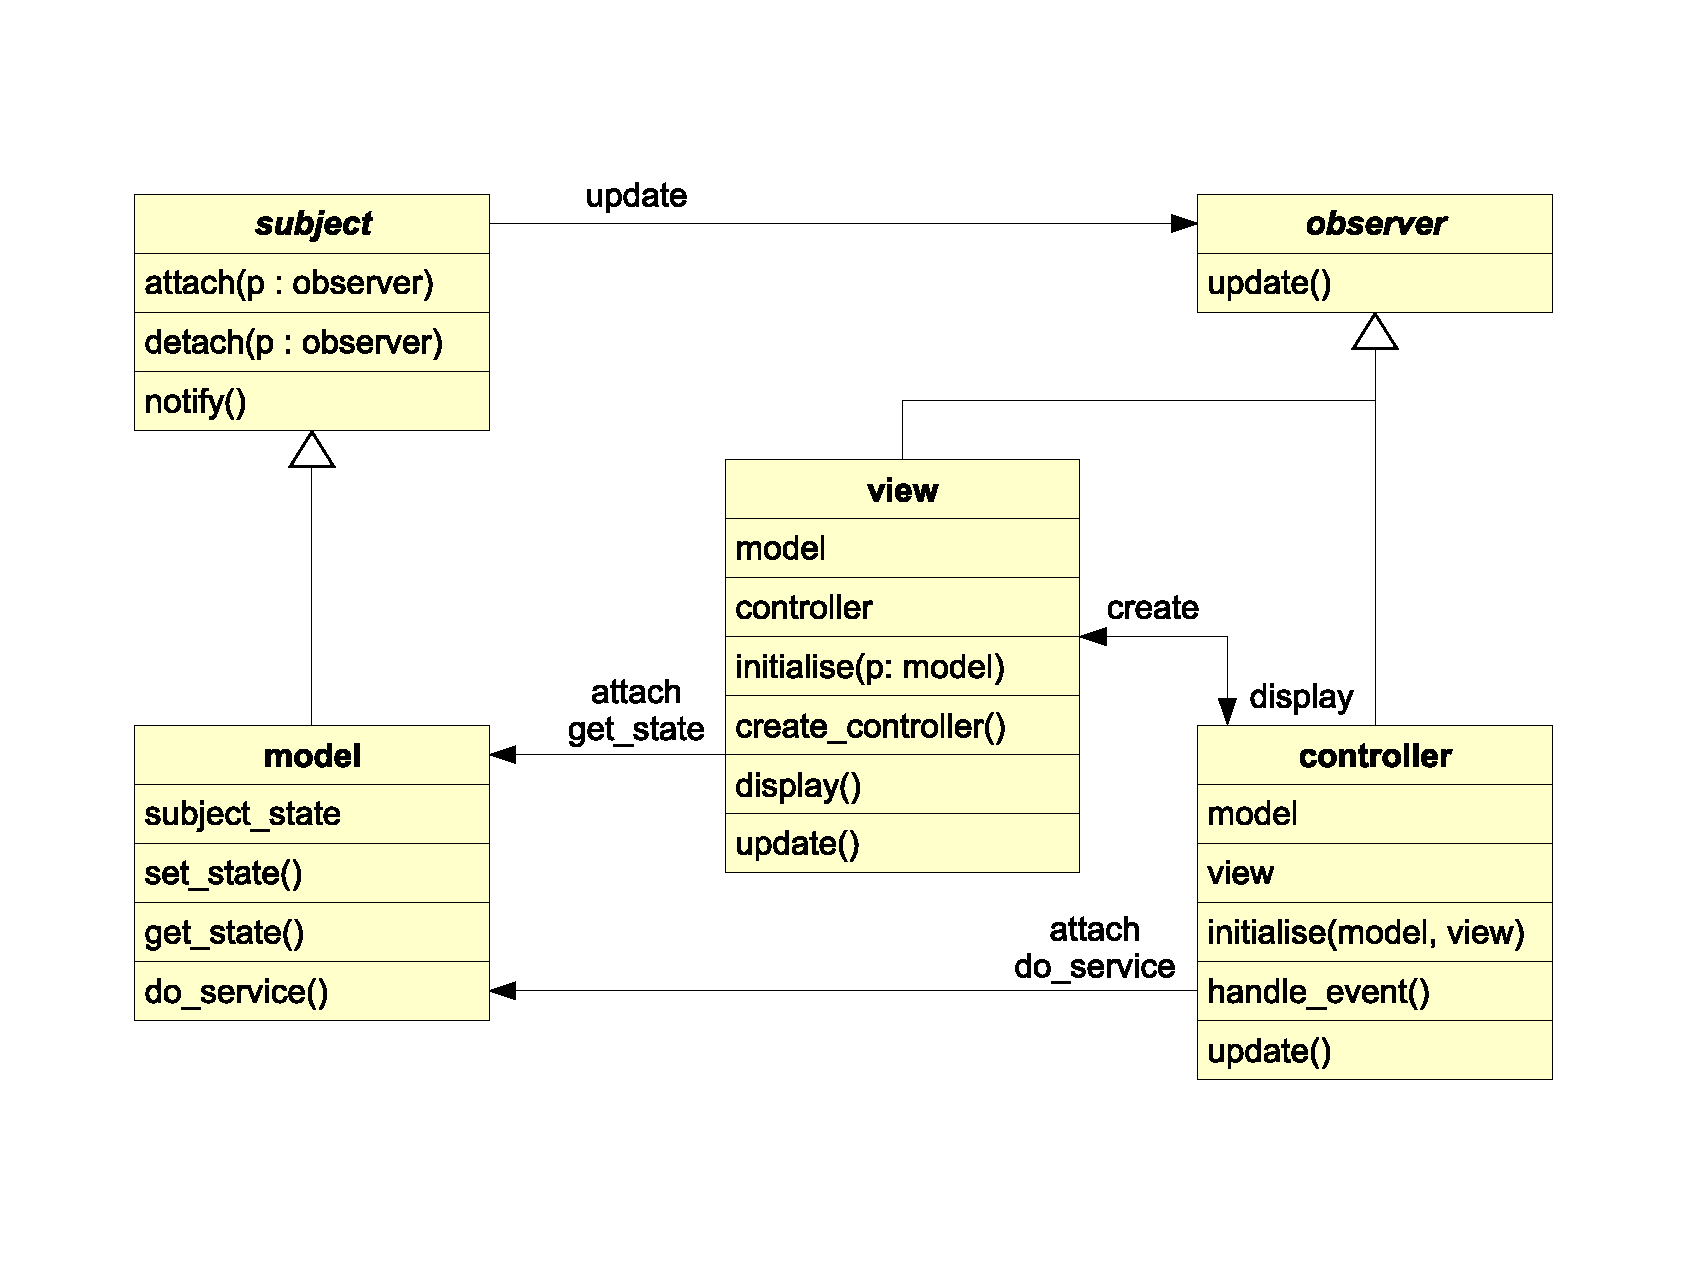
\includegraphics[scale=0.3]{vector/mvcobserver.eps}
        \caption{MVC- using Observer Pattern}
        \label{mvcobserver_figure}
    \end{center}
\end{figure}

Similar notification mechanisms are used for \emph{Callback} event handling in
frameworks, where the framework core calls functionality of its extensions. The
\emph{Model View Controller-} (MVC) uses the \emph{Observer} pattern to let the
model notify its observing views about necessary updates (figure
\ref{mvcobserver_figure}).

A disadvantage of the \emph{Observer} pattern is that it relies on bidirectional
dependencies (section \ref{bidirectional_dependency_heading}), so that circular
references can occur, when a system is not programmed very carefully.

